\chapter{The model}
\label{chap:growing}

We model the economy as a network of interacting firms whose sizes evolve by Generalized
Lotka--Volterra dynamics. We choose these dynamics because they are the least we can assume about
a large collection of firms that each grow on their own and interact in pairs, with every firm
carrying its own logistic growth and self-limitation and every competitive or cooperative link a
single entry of a signed interaction matrix. This is the natural model of a large disordered
community, the same one used for interacting species in theoretical ecology \citep{may1972}. The standard form of these dynamics cannot represent
a growing economy, and this chapter builds the model that can by changing the standard form one
step at a time, fixing each defect as it appears. The result is then analysed in
Section~\ref{sec:model-phases}, where we locate the growing, fluctuating regime in which the
firm-growth statistics of Chapter~\ref{chap:firmgrowth} are measured.

\section{From Lotka--Volterra to the relative model}
\label{sec:relative-model}

\subsection{The starting point and why it fails}
\label{sec:starting-point}

We take as our starting point the Generalized Lotka--Volterra (GLV) system for $N$ firms. Each
firm $i$ carries a size $x_i \ge 0$ that grows logistically and is coupled to the others through a signed
interaction matrix,
\begin{equation}
    \dot{x}_i = x_i \left( 1 - x_i + (Wx)_i \right),
    \label{eq:abs-glv}
\end{equation}
with $W_{ij} = A_{ij}\,\alpha_{ij}$ on a sparse configuration-model graph with a broad, power-law
degree distribution. Here $A_{ij}$ is the
adjacency matrix of the graph, $1$ where firms $i$ and $j$ are connected and $0$ otherwise, and
$C$ is the mean degree. The coupling strength on each edge is usually taken to be
\begin{equation}
    \alpha_{ij} = \frac{\mu}{C} + \frac{\sigma}{\sqrt{C}}\,z_{ij},
    \label{eq:coupling-global}
\end{equation}
with the $z_{ij}$ independent standard Gaussian variables, drawn once for each graph and then held
fixed, the quenched disorder of the model. The first term is a fixed mean interaction, cooperative
for $\mu > 0$ and competitive for $\mu < 0$, and the second is a random part of size $\sigma$ that
makes every link different. Both are divided by the mean degree so that the pressure a firm feels
stays of order one as the graph is made denser, since a firm with about $C$ neighbours picks up a
mean of order $C \cdot \mu/C = \mu$ and, summing $C$ independent random terms, a spread of order
$\sqrt{C}\,\sigma/\sqrt{C} = \sigma$.

Equation~\eqref{eq:abs-glv} cannot serve as it stands, and it fails for two reasons. The first is
that it carries an absolute scale of size that an economy does not have, since the self-limitation
$-x_i$ caps an isolated firm at $x_i = 1$ and the quadratic interaction fixes once and for all the
size at which growth, competition and self-limitation balance. A real economy has no such
reference size. Its output has grown by orders of magnitude over two centuries while the
distribution of firm sizes and the statistics of their growth stayed essentially stationary, so
the dynamics should be invariant under a rescaling $x \to c\,x$ of the whole economy, which
\eqref{eq:abs-glv} is not. The absolute model can be made to grow without bound, but only by
tuning the cooperation to the critical strength at which its bounded fixed point disappears, and
there the total abundance diverges in finite time rather than growing steadily.

The second reason is that even at that point the absolute model delivers only one of the two
firm-growth facts we are after, since it reproduces the fat-tailed growth-rate distribution on
heterogeneous graphs, but its size--variance relation is not a stationary law, only a transient
traced out as an arbitrary initial condition relaxes onto the critical attractor, after which
every growth rate vanishes. We need, then, two things the absolute model lacks, invariance under
rescaling and a state that keeps fluctuating rather than relaxing.

\subsection{The relative model}
\label{sec:relative-derivation}

Scale invariance alone fixes the form of the change. For the dynamics to be unchanged under
$x \to c\,x$ the right-hand side of \eqref{eq:abs-glv} must be homogeneous of degree one in $x$,
and while the growth term $x_i$ already is, the self-limitation $x_i^2$ and the interaction
$x_i (Wx)_i$ are both of degree two. To bring them back to degree one we divide each by a quantity
that scales like a size, and the natural one is the average firm $m = \langle x\rangle$, the
typical firm that each one competes against. One further term completes the model. Left to
itself the chaotic flow drives some firms arbitrarily close to zero size, and a firm that
reaches zero stays there, so diversity erodes and the state never becomes stationary. As is
standard in the disordered Lotka--Volterra literature \citep{bunin2017,roy2020} we add a small
immigration term, an entry flow of small firms at a rate set by the size of the economy itself,
which prevents exact extinction. The model of this thesis is then, in its entirety,
\begin{equation}
    \dot{x}_i \;=\; x_i \left( 1 - \frac{x_i}{m} + \frac{(Wx)_i}{m} \right)
    \;+\; \lambda\,( m - x_i ),
    \qquad m = \frac{1}{N}\sum_j x_j ,
    \label{eq:relative-glv}
\end{equation}
with $W_{ij} = A_{ij}\,\alpha_{ij}$ the disordered couplings \eqref{eq:coupling-global} on the
scale-free graph, and $\lambda = 10^{-3}$ the immigration rate. The immigration term reads as
entry plus turnover: split as $+\lambda m - \lambda x_i$, it is a constant influx of small firms
at rate $\lambda m$ together with a uniform exit of every firm at rate $\lambda$, and it sums to
zero over the economy, so it reshuffles mass without changing the total. Although it nominally
pulls firms above the mean downward, its per-capita effect on a large firm is bounded by
$\lambda = 10^{-3}$, uniform across all large firms and three orders of magnitude below the
interaction-driven fluctuations, so it cannot tilt the size-conditioned statistics; where it
bites is at the bottom, where the influx $\lambda m$ outlives the vanishing multiplicative terms
and sets the floor that keeps firms from exact extinction --- its entire measurable footprint is
the small-firm plateau excluded from the fits of Chapter~\ref{chap:firmgrowth}. The only changes
from the
standard system \eqref{eq:abs-glv} are the two factors of $1/m$ and the immigration term, and
every term is now homogeneous of degree one: under $x \to c\,x$ the mean $m$ scales the same
way, the ratios $x_i/m$ and $(Wx)_i/m$ are unchanged, the immigration flow $\lambda(m - x_i)$
rescales with the economy, and so if $x(t)$ is a solution then so is $c\,x(t)$. The economy no
longer has a preferred size. The change
is also the economically natural one, since a competitor's pressure on firm $i$ is now set by its
market share $x_j/m$ rather than by its absolute size, and a firm's own crowding is measured
against the typical firm rather than against a fixed ceiling, so what drives the dynamics is
relative standing in the market. The intrinsic Malthusian rate $1$ is left untouched and remains
the engine of growth, while the interactions, now made relative, only regulate it.

\subsection{The couplings and the graph}
\label{sec:completing-model}

The couplings retain the standard normalization \eqref{eq:coupling-global}: every edge is divided
by the (realized) mean degree $C$, the same for every firm, exactly as in the disordered
Lotka--Volterra literature. The graph is a configuration model with a power-law degree
distribution of exponent $2.5$. On such a heterogeneous graph the standard normalization has a
consequence on which the results of Chapter~\ref{chap:firmgrowth} will turn: a firm with $k_i$
neighbours sums $k_i$ independent couplings of variance $\sigma^2/C$, so the variance of the
disorder field it feels grows with its own connectivity, $\mathrm{Var}\,h_i \propto k_i/C$. The
degree distribution of the graph is thereby printed onto the distribution of firm-level
noise --- hubs live in louder environments --- and this is the channel through which the
topology reaches the firm-growth statistics. (An alternative, which an earlier stage of
this work explored, normalizes each firm by its own degree,
$\alpha_{ij} = \mu/k_i + (\sigma/\sqrt{k_i})\,z_{ij}$, equalizing the field variance
across firms; Chapter~\ref{chap:firmgrowth} shows that this cancels the graph out of the
size-conditioned statistics and with it the multiscaling, so we set it aside.)

Under the standard normalization the mean degree must scale with the system,
$C \propto N$, the usual dilute-coupling prescription whose fully-connected limit is the
$C = N$ Gaussian ensemble; we hold the dilution fixed at $C = N/40$. On the power-law
graph this keeps the whole degree hierarchy at fixed fractions of $N$ --- the largest hub
saturates the natural cutoff at $k \approx N$, and the over-coupling of the hubs relative
to the mean, of order $k_{\max}/C = N/C$, stays finite as the economy grows. At fixed $C$,
by contrast, the hub over-coupling grows without bound and the size--variance law washes
out with system size.

\subsection{A convenient change of variables}
\label{sec:growth-churn}

Because the model is scale-invariant, a firm's size matters only relative to the average
firm, and the convenient variables are exactly the ones the data use: the scale of the
economy, and each firm's size in units of that scale,
\begin{equation}
    S_i = \frac{x_i}{m}, \qquad \langle S \rangle = 1,
\end{equation}
where $\langle\,\cdot\,\rangle$ denotes the average over firms. The relative sizes carry
the composition of the economy, their mean pinned to one by construction, and the average
firm $m$ carries its overall scale. The split separates the two things the model does, and
no system-size factor appears in either piece.

The scale grows steadily. Averaging \eqref{eq:relative-glv} over firms, the immigration
term drops (it conserves the total), and
\begin{equation}
    \dot{m} = m\, g_{\mathrm{eff}},
    \qquad
    g_{\mathrm{eff}} = \langle S f \rangle
                     = 1 + \langle S\,(WS) \rangle - \langle S^2 \rangle ,
    \label{eq:Mdot-relative}
\end{equation}
the size-weighted average fitness of the firms. Averaging the absolute model
\eqref{eq:abs-glv} instead leaves a right-hand side quadratic in the scale, the feedback
responsible for the finite-time singularity, whereas dividing the interactions by $m$
removes one power of it, so \eqref{eq:Mdot-relative} is the equation of exponential
growth, with no singularity. The rate
$g_{\mathrm{eff}}$ fluctuates as the composition churns, but its time-average is a small
positive constant, so $\log m$ climbs at a steady slope over unbounded time.

The composition, by contrast, never settles. From \eqref{eq:relative-glv} and the quotient
rule the relative sizes obey
\begin{equation}
    \begin{gathered}
        \dot{S}_i = S_i \left( f_i - g_{\mathrm{eff}} \right)
                    + \lambda\,( 1 - S_i ), \\
        f_i = 1 - S_i + (WS)_i ,
    \end{gathered}
    \label{eq:replicator}
\end{equation}
with the linear fitness $f_i$ and the same size-weighted average
$g_{\mathrm{eff}} = \langle S f\rangle$ as in \eqref{eq:Mdot-relative}, so the economy
grows at the average fitness of its firms. This is a
replicator equation, the canonical description of frequency-dependent selection in which a
firm gains relative size precisely when its fitness exceeds the market average, plus the
immigration flow pulling each firm toward the mean size one; it is
the standard correspondence between Lotka--Volterra and replicator dynamics
\citep{hofbauer81}. Note that $N$ appears nowhere in
\eqref{eq:Mdot-relative}--\eqref{eq:replicator}: the number of firms enters the model only
through the construction of the couplings (the graph and its mean degree $C = N/40$) and
as the number of degrees of freedom, not through the form of the dynamics.
Because the relative model does not blow up, these equations are written in the same
physical time $t$ in which
$m$ grows, with no time rescaling. Above the disorder threshold $\sigma_c$
\citep{diederich1989,opperdiederich1992} the replicator flow does not relax to a fixed
point but stays chaotic, so
the growth rates never vanish, which is the persistently fluctuating state we needed.

The practical payoff of the split is numerical. We integrate \eqref{eq:replicator}
together with $\mathrm{d}\ln m/\mathrm{d}t = g_{\mathrm{eff}}$
directly in physical time, keeping the composition in its bounded variables (the relative
sizes have fixed mean one) and the scale in its
logarithm, so nothing overflows however large $m$ becomes even though the economy grows by
many orders of magnitude over a run; the explicit solver and its cost
are specified in Appendix~\ref{app:numerics}.

Figure~\ref{fig:growing-churn} shows a single run in this regime. The total abundance
(left)
climbs as a straight line in its logarithm over the whole integration, the steady
exponential growth
of \eqref{eq:Mdot-relative}, with no sign of a blow-up. The relative firm sizes
$S_i = x_i/m$ (right) do not settle; after an initial transient they
keep exchanging rank and spanning orders
of magnitude, the persistent chaos of the $\sigma > \sigma_c$ phase. The economy grows
while its
composition keeps turning over.

\begin{figure}[htbp]
    \centering
    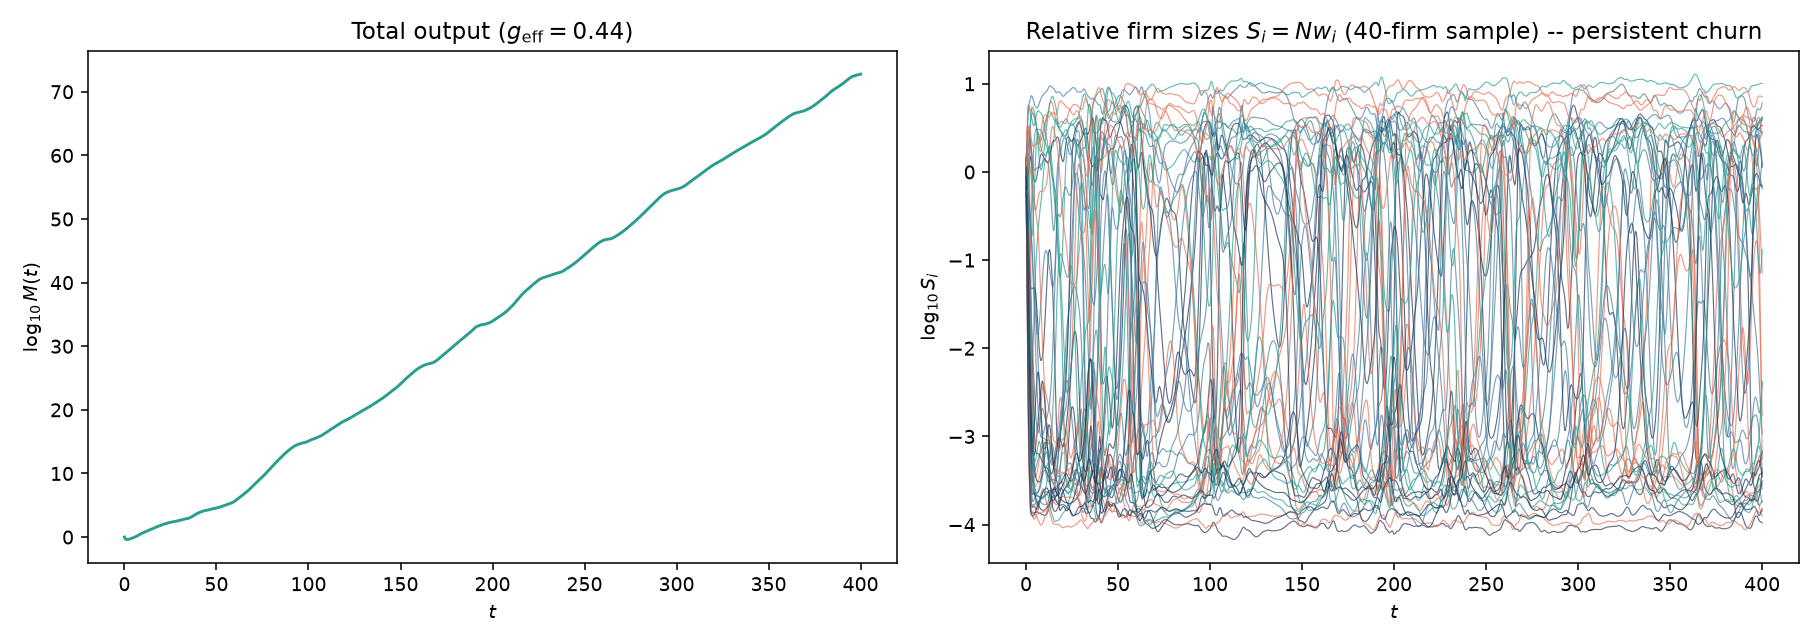
\includegraphics[width=\linewidth]{growing_growth_churn.png}
    \caption{A single run of the relative model \eqref{eq:relative-glv} at $\mu = -1.76$,
    $\sigma = 1.75$, $\lambda = 10^{-3}$ on a power-law graph with $N = 6400$. \panel{Left}: the
    total abundance grows exponentially in physical time, its logarithm rising
    linearly, with no finite-time divergence. \panel{Right}: a sample of relative firm sizes
    $S_i = x_i/m$, which keep fluctuating and exchanging rank rather than relaxing to a
    fixed point.}
    \label{fig:growing-churn}
\end{figure}

\section{Phases of the model}
\label{sec:model-phases}

Before measuring the firm-growth statistics it helps to see where in parameter space the
growing, fluctuating state lives. Figure~\ref{fig:phase-diagram} maps the behaviour of the model
over the plane of the mean interaction $\mu$ and the disorder $\sigma$, classified from the
late-time dynamics of many graph realizations. Two genuine transitions organize it. The
dynamical threshold $\sigma_c$ separates a frozen regime below, where the shape
relaxes to a fixed point and the growth rates vanish, from the chaotic regime above, where it
never settles. Cutting across it, the line $g_{\mathrm{eff}} = 0$ separates a growing economy
from a shrinking one. Where the competition is strong and the disorder high, coexistence
collapses and the dynamics either condense onto a few firms or grow explosively.

The regime we want is pinned down by three things the data demand, and each one rules out part of
the plane. The economy must grow, since output has risen for two centuries, which requires
$g_{\mathrm{eff}} > 0$ and discards the whole shrinking half below the $g_{\mathrm{eff}} = 0$ line.
Its firms must keep growing period after period, so that firm growth is a stationary statistic
rather than a one-off event, and this requires the chaotic phase above $\sigma_c$, since in the
frozen phase below it the shape relaxes to a fixed point and every growth rate vanishes, leaving
the same transient size--variance relation that already ruled out the absolute model. The economy
must also stay diverse, a whole distribution of coexisting firms, which discards the
strong-competition, high-disorder corner where coexistence collapses onto a handful of firms or
the sizes diverge. What survives all three demands is the chaotic, growing band, where the model reproduces the
empirical firm-growth statistics of Moran, Secchi and Bouchaud \citep{moran2024}, the region
labelled MSB in Figure~\ref{fig:phase-diagram}. It is the wedge bounded below by $\sigma_c$, on
the competitive side by the $g_{\mathrm{eff}} = 0$ line, and on the strong-disorder side by the
condensed corner. It is an extended region rather than an isolated point, so what follows
describes the behaviour of the model and not a single tuned operating point.

\begin{figure}[htbp]
    \centering
    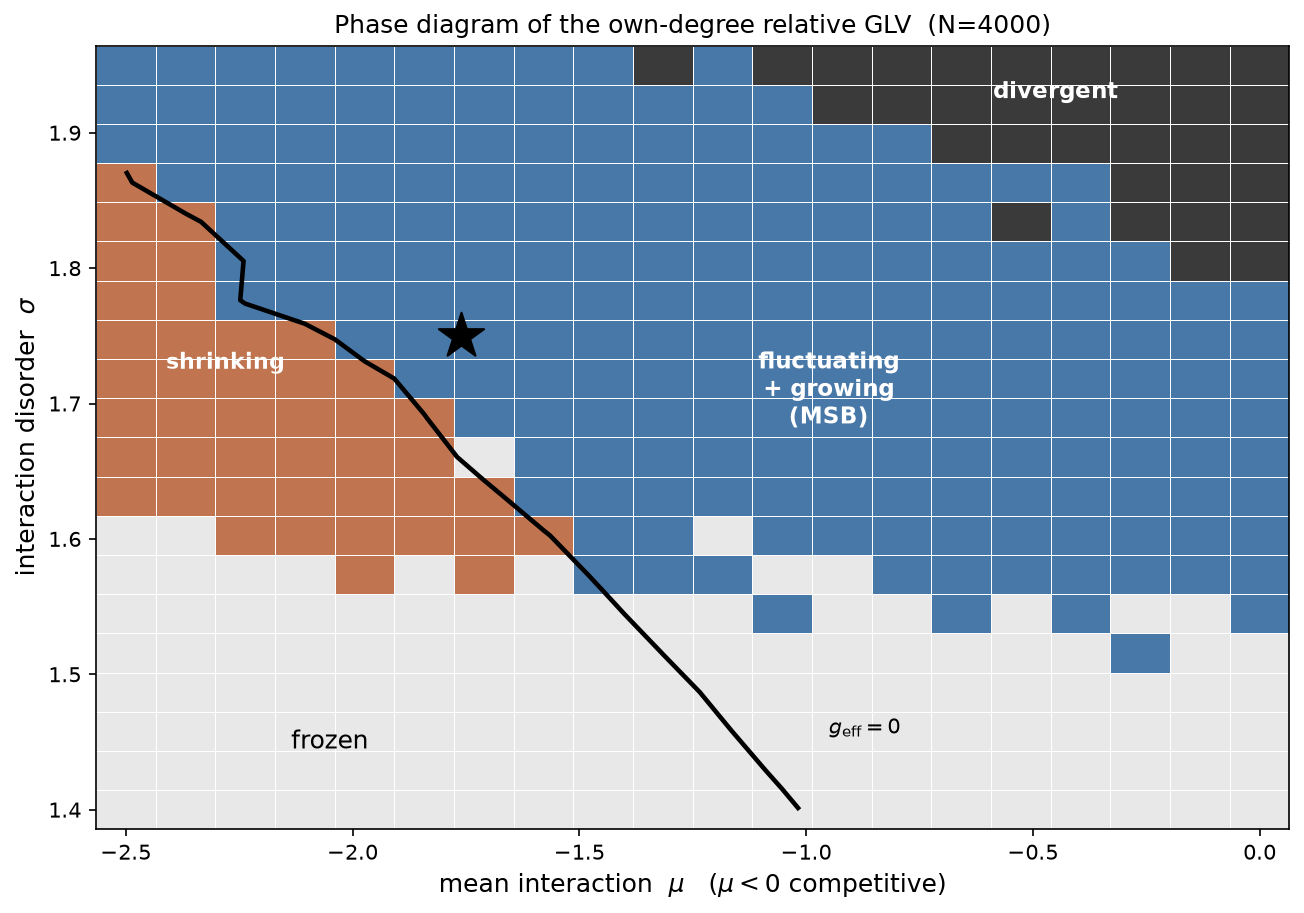
\includegraphics[width=\linewidth]{phase_diagram.png}
    \caption{Phase diagram of the relative model \eqref{eq:relative-glv}, over the mean
    interaction $\mu$ (competitive for $\mu < 0$)
    and the disorder $\sigma$, classified from the late-time dynamics ($N = 4000$, a
    $20 \times 20$ grid with ten realizations per cell). The diagram was mapped under the
    per-firm normalization noted in Section~\ref{sec:completing-model}; under the standard
    normalization used throughout this thesis the same qualitative structure holds but the
    fluctuating band is somewhat narrower --- at the operating point every realization at
    $N \ge 8000$ persists (Chapter~\ref{chap:firmgrowth}), while stronger disorder
    ($\sigma = 2.0$) already loses most realizations to the collapsed corner. At low disorder the shape relaxes and nothing fluctuates
    (frozen). Above it the dynamics are chaotic, and the solid black line marks the growth
    boundary $g_{\mathrm{eff}} = 0$, which separates the shrinking region ($g_{\mathrm{eff}}
    < 0$) from the fluctuating, growing band in which the firm-growth statistics are
    measured (blue, labelled MSB, for Moran--Secchi--Bouchaud). The band is bounded below by the
    freezing line, on the competitive side by $g_{\mathrm{eff}} = 0$, and in the strong-disorder corner by the
    explosive, divergent region. The star marks the operating point $\mu = -1.76$,
    $\sigma = 1.75$. The band is an extended region rather than a single point.}
    \label{fig:phase-diagram}
\end{figure}

This phase structure has a mean-field underpinning. The relative model
\eqref{eq:relative-glv} is a disordered replicator equation, and its dynamical mean-field theory,
worked out in Appendix~\ref{app:dmft}, reduces the $N$-firm dynamics to a single representative
firm in a self-consistent Gaussian field. This is the standard replicator mean-field
\citep{galla2018,roy2020}, whose chaos transition is the mean-field counterpart of the freezing
line. Below it the shape relaxes to a fixed point and the growth rates vanish, above it the flow
never settles. The mean interaction enters every firm's fitness as the same uniform shift, so it
cancels from the replicator and only sets the level of the growth rate $g_{\mathrm{eff}}$, moving
the $g_{\mathrm{eff}} = 0$ line but not the freezing threshold. We locate the threshold and
measure the firm-growth statistics directly from the simulations.
